\documentclass{article}
\usepackage[utf8]{inputenc}
\usepackage[T1]{fontenc}
\usepackage{graphicx}
\usepackage{hyperref}
\usepackage{geometry}
\geometry{margin=1in}

\title{SILLIUS TALIOLOS}
\date{Encyclopaedia Britannica (1771)}

\begin{document}
\maketitle

\section*{Historical source}
\textbf{Entry ID:} \texttt{entry-sillius-taliolos-2001} \\
\textbf{Volume ID:} 192200899 \\
\textbf{Character Count:} 1022

\subsection*{Extracted Text}
SILLIUS TALIOLOS, CAUS, an ancient Roman poet, and author of an epic poem in 17 books, which con-tains an hilloy of the second Ponte was, to famous for having decided the empire of the world in favour of the Romanes. He was born in the reign of Thierius, and is fogoped to have derived the name of \_Italica\_ from the place of his birth; but whether he was born at Italica in Spain, or at Cerdinam in Italy, which, according to Scheba, had the name of \_Italica\_ given it during the Social war, is a point which cannot be known: though, it is his first had happened at either of those places, the grammarina would tell us, that he found have been called \_Italicaeta\_, and wol \_Italica\_. When he came to Rome, he applied himself to the bay; and, by a choi institution of Greece, succeeded fo well, like he became a celebrated advocate and molt accomplished senior. His sacred, and charader recommended him to the high- ethnics in the republic, even to the confidity, of which he was poffied when Nono died. He is field to Yγ2



\section*{Source record}
\begin{itemize}
\item \textbf{Dataset:} \texttt{NationalLibraryOfScotland/encyclopaedia\_britannica\_illustrated}
\item \textbf{Dataset Revision:} \texttt{309f765b1ecc83e0a7f7762e44b4a927a7555443}
\item \textbf{Page ID:} \texttt{britannica:309f765b1ecc83e0a7f7762e44b4a927a7555443:train:2001} \\
  \textbf{Filename:} \texttt{page-2001-93040a5ab362.jpg} \\
  \textbf{Row Index:} 2001 \\
  \textbf{SHA256:} \texttt{93040a5ab3625efc...}
\end{itemize}

\begin{figure}[h]
\centering
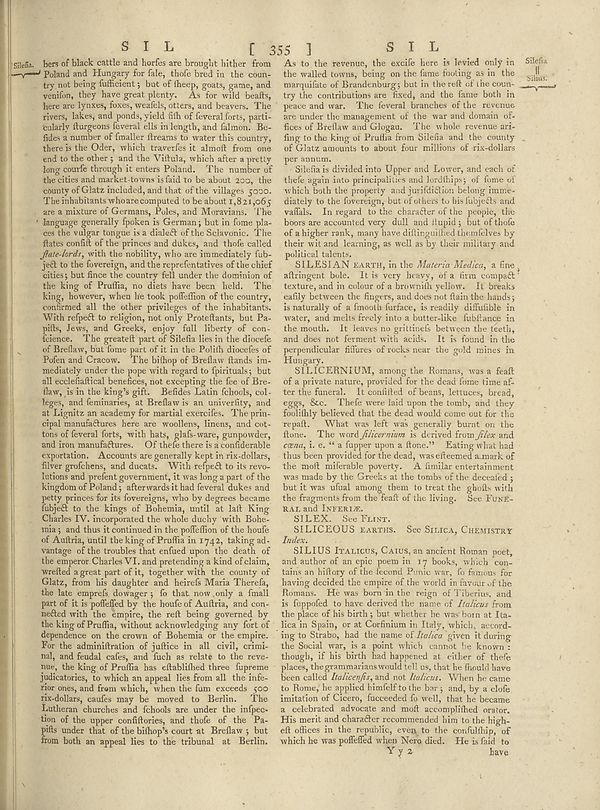
\includegraphics[width=0.85\textwidth]{../scans/page-2001-93040a5ab362.jpg}
\caption*{Source scan: \texttt{page-2001-93040a5ab362.jpg}}
\end{figure}

\end{document}
